\chapter{\IfLanguageName{dutch}{Testopstelling/PoC}{Test/PoC}}%
\label{ch:onderzoek}

\section{\IfLanguageName{dutch}{Opzetten testopstelling}{Creating test environment}}%
\label{sec:testopstelling}

Voor het opzetten van de testopstelling is een gratis trial aangegaan voor elk van de gekozen vijf databases. Deze omvatten: MariaDB, ClickHouse, Couchbase, Amazon Aurora en MongoDB Atlas.

Door het bedrijf Aware werd een statistiek ter beschikking gesteld met betrekking tot de uitgevoerde queries. Dit wordt weergegeven in figuur~\ref{fig:statistics}.

\begin{figure}[H]
    \centering
    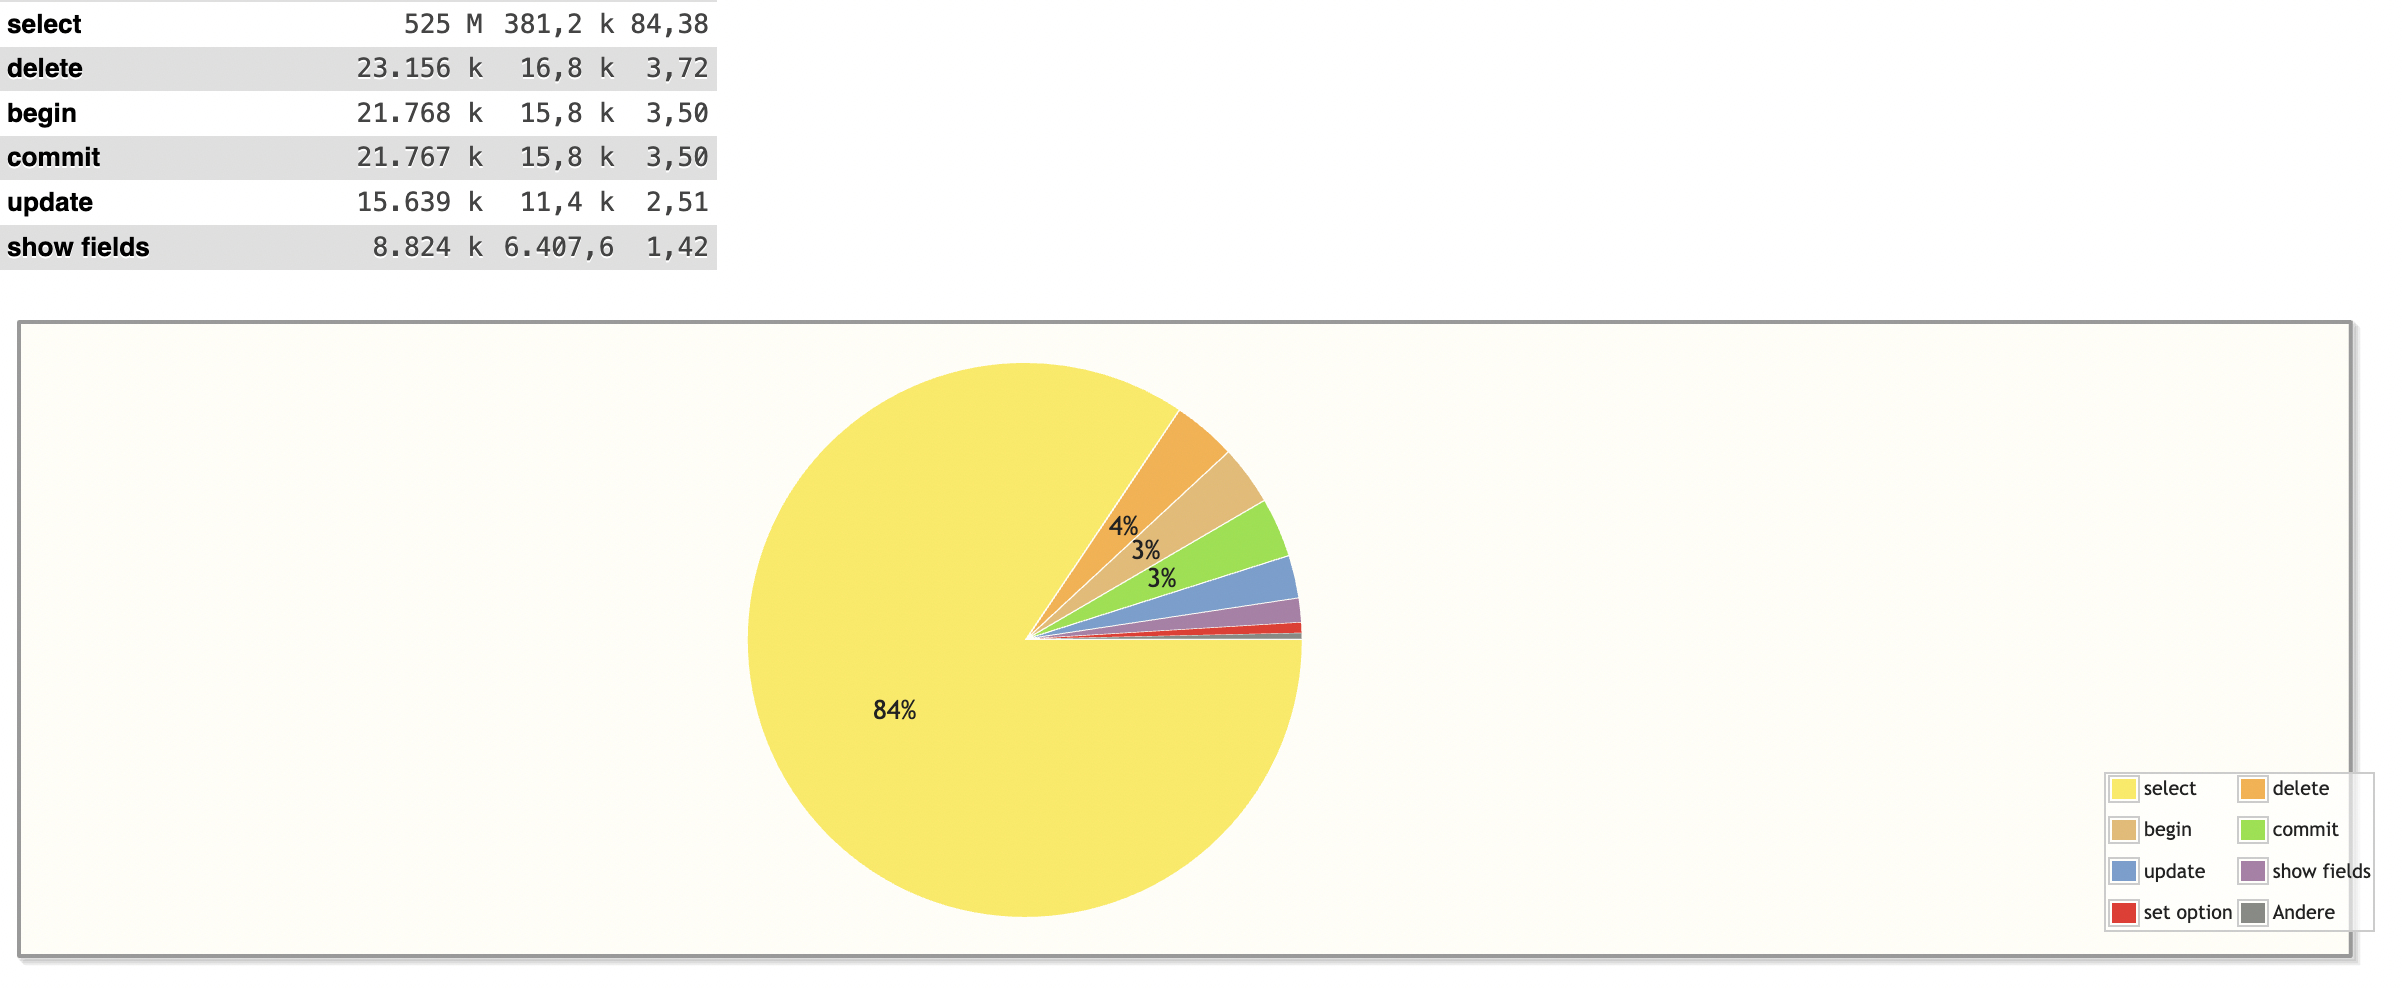
\includegraphics[width=\linewidth]{graphics/statistics}
    \caption[Query statistieken Aware]{Query statistieken Aware | mei 2023 - maart 2024}
    \label{fig:statistics}
\end{figure}

Op basis van verkregen statistieken van het bedrijf Aware, kan afgeleid worden dat het merendeel van de uitgevoerde queries, select queries zijn. Tijdens het testen zal hier dan ook de nadruk op gelegd worden. 

Voor het testen van de database prestaties is het belangrijk te definiëren welke statistieken gemeten en gemonitord moeten worden. Tijdens de testen zal er vooral gefocust worden op de response time, de tijd die de database erover doet om een query of een transactie uit te voeren en de gevonden resultaten terug te geven aan de gebruiker. 

Zoals eerder besproken in de stand van zaken wordt er vanuit gegaan dat een e-commerce webshop in de mode-industrie volgende gegevens opslaat: 

\begin{itemize}
    \item Klanten
    \item Producten
    \item Categorieën
    \item Bestellingen
    \item Bestelitems
    \item Betaalmethoden
    \item Verzendmethoden
    \item Voorraad
    \item Logs
\end{itemize}
Om de database op te vullen met deze gegevens werd er random data gegenereerd voor deze gegevens.

\newpage

\section{\IfLanguageName{dutch}{MariaDB}{MariaDB}}%
\label{sec:test-mariadb}

\subsection{\IfLanguageName{dutch}{Opzetten van de database}{Creating the database}}%
\label{subsec:creating-mariadb}

Nadat de MariaDB-client is geïnstalleerd, werd een terminal geopend waarin enkele commando's werden uitgevoerd om een nieuwe database aan te maken. In Figuur~\ref{fig:mariadbconnection} wordt een dergelijke terminal geïllustreerd waarin al een verbinding met de MariaDB-client is gemaakt.

\begin{figure}[H]
    \centering
    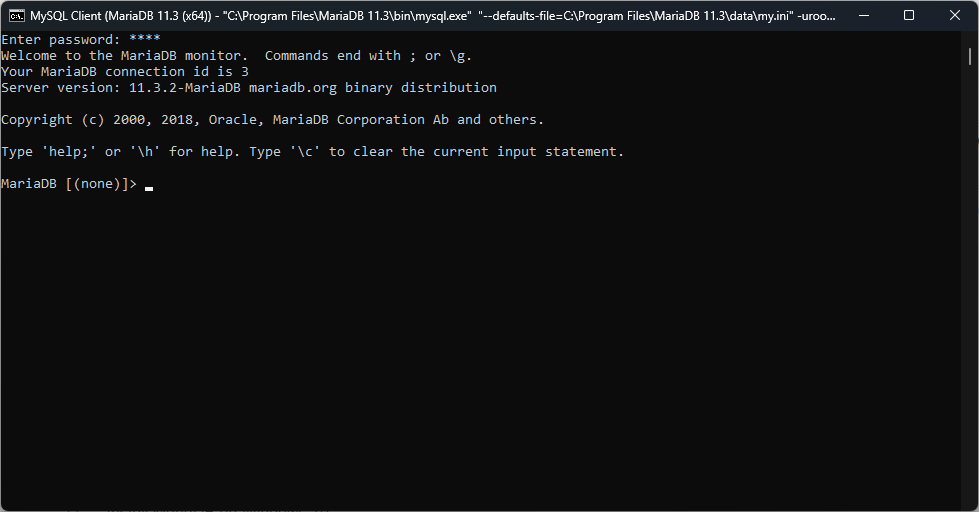
\includegraphics[width=\linewidth]{graphics/mariadbconnection}
    \caption[Terminal met een actieve verbinding met de MariaDB-client.]{Terminal met een actieve verbinding met de MariaDB-client.}
    \label{fig:mariadbconnection}
\end{figure}

Er kan een database in de MariaDB-client worden aangemaakt door volgend commando uit te voeren:

\begin{lstlisting}[language=SQL, caption={SQL-query voor het aanmaken van de database.}]
    CREATE DATABASE mariadbtest;
\end{lstlisting}

Voor het opstellen van het schema van de database werd vooraf een eenvoudig Entity-Relationship Diagram (ERD) opgesteld, zoals te zien is in Figuur~\ref{fig:erd-e-commerce}. Dit ERD diende als basis voor het opstellen van de database.

\begin{figure}[H]
    \centering
    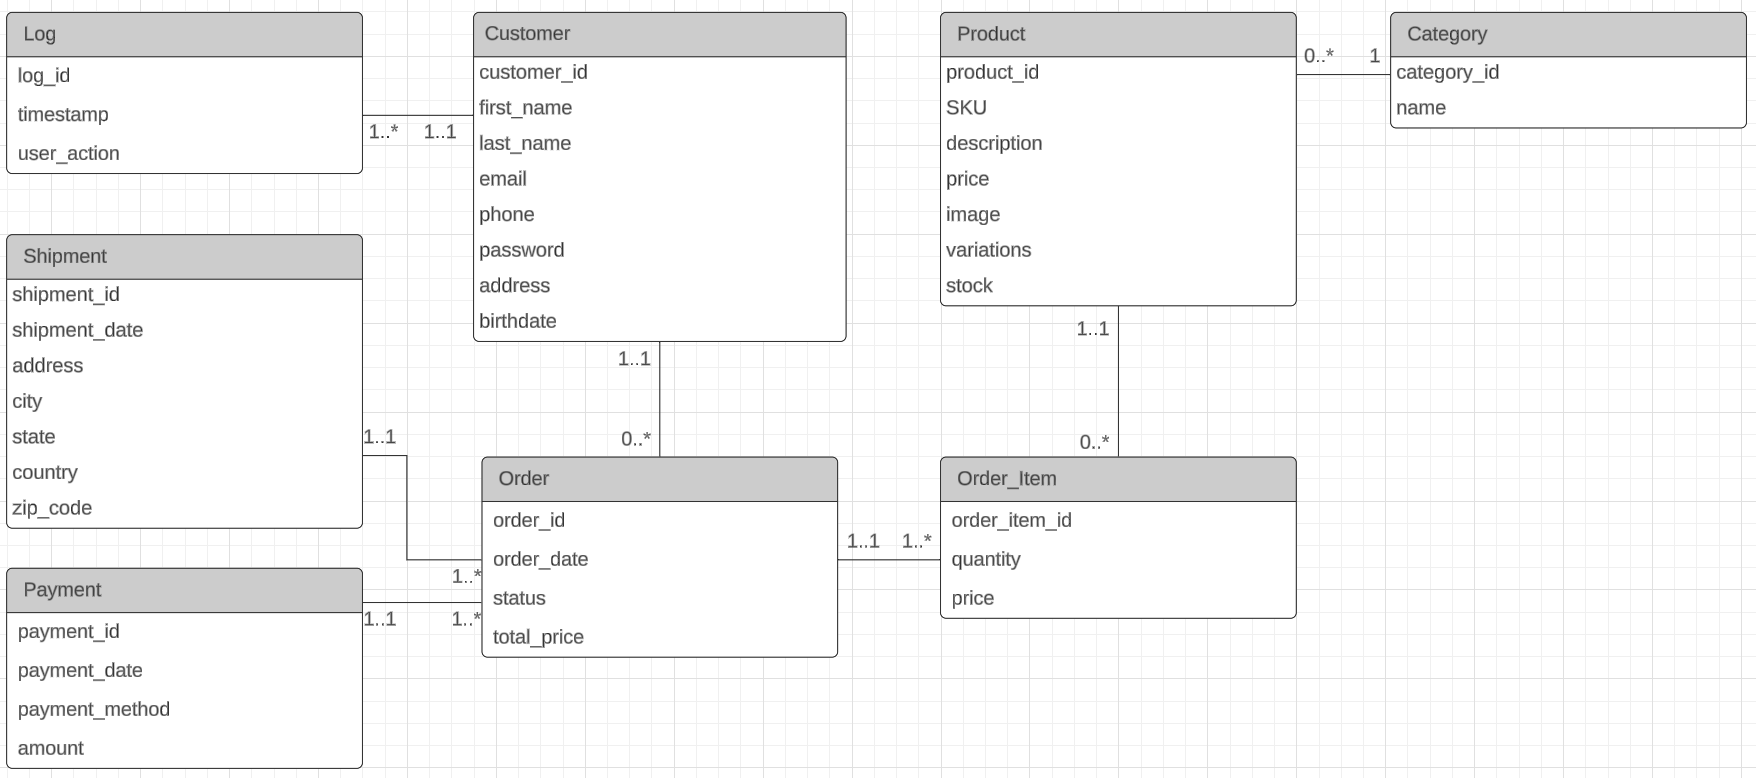
\includegraphics[width=\linewidth]{graphics/erd-e-commerce}
    \caption[Entity-Relationship Diagram (ERD) voor het e-commerce project.]{Entity-Relationship Diagram (ERD) voor het e-commerce project.}
    \label{fig:erd-e-commerce}
\end{figure}

Om de tabellen in de database te maken, werden volgende commando's uitgevoerd:

\begin{lstlisting}[language=SQL, caption={SQL-queries voor het aanmaken van de categorie en product tabel in de database.}]
    CREATE TABLE Category (
    category_id INTEGER AUTO_INCREMENT,
    name VARCHAR(50) NOT NULL,
    PRIMARY KEY (category_id)
    );
    
    CREATE TABLE Product (
    product_id INTEGER AUTO_INCREMENT,
    category_id INTEGER,
    SKU VARCHAR(50),
    description VARCHAR(255),
    price DECIMAL(10, 2),
    stock INTEGER,
    image VARCHAR(255),
    variations JSON,
    PRIMARY KEY (product_id),
    FOREIGN KEY (category_id) REFERENCES Category(category_id)
    );
\end{lstlisting}

Na het uitvoeren van alle commando's werd een schema zoals weergegeven in Figuur~\ref{fig:mariadb} verkregen.

\begin{figure}[H]
    \centering
    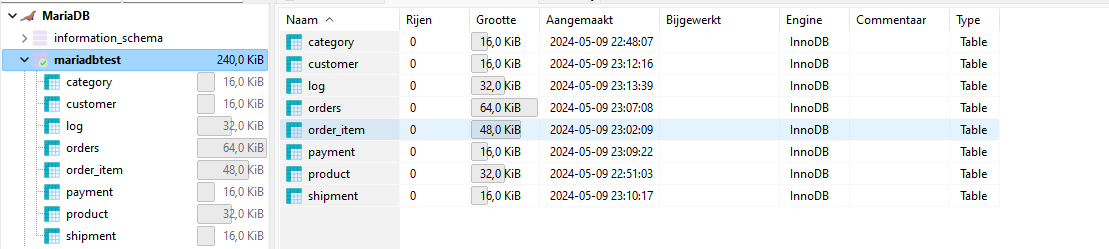
\includegraphics[width=\linewidth]{graphics/mariadb}
    \caption[Schema van de database na het aanmaken van de tabellen.]{Schema van de database na het aanmaken van de tabellen.}
    \label{fig:mariadb}
\end{figure}

Voordat er testen kunnen worden uitgevoerd, moet er data in de database worden ingevoerd. Dit kan met behulp van het volgende commando:

\begin{lstlisting}[language=SQL, caption={SQL-query voor het invoegen van nieuwe categorieën in de database.}]
    INSERT INTO Category (name) VALUES
    ('Kleding'),
    ('Schoenen'),
    ('Accessoires'),
    ('Handtassen'),
    ('Sieraden'),
    ('Horloges'),
    ('Sportkleding'),
    ('Zwemkleding'),
    ('Ondergoed'),
    ('Nachtkleding'),
    ('Werkkleding'),
    ('Feestkleding'),
    ('Casual kleding'),
    ('Vintage kleding'),
    ('Duurzame kleding'),
    ('Plus-size kleding'),
    ('Kinderkleding'),
    ('Babykleding'),
    ('Herenkleding'),
    ('Dameskleding');
\end{lstlisting}

Nadat er voldoende data ($\pm$ 3.8 miljoen rijen) is geïmporteerd, kunnen er testen worden uitgevoerd. Als voorbeeld wordt een SELECT-query uitgevoerd om alle producten te tonen die zijn geassocieerd met de categorie "Schoenen", gevolgd door een query om een schoen bij te werken, toe te voegen en te verwijderen.

\begin{lstlisting}[language=SQL, caption={SQL-queries voor het beheren van producten in de database.}]
    -- Query 1: Ophalen van alle producten voor een bepaalde categrorie.
    SELECT p.product_id, p.SKU, p.description, p.price, p.stock,
     p.image, c.name AS category_name
    FROM Product p
    JOIN Category c ON p.category_id = c.category_id
    WHERE c.name = 'Schoenen';
    
    -- Query 2: Update van een product
    UPDATE Product
    SET description = 'Nieuwe beschrijving', price = 49.99, stock = 100
    WHERE product_id = 1;
    
    -- Query 3: Toevoegen van een nieuw product
    INSERT INTO Product 
    (category_id, SKU, description, price, stock, image, variations)
    VALUES 
    (1, 'SKU123', 'Nieuw product', 39.99, 50, 'product_image.jpg', 
    '{"size": "L", "color": "blue"}');
    
    -- Query 4: Verwijderen van een product
    DELETE FROM Product
    WHERE product_id = 2;
\end{lstlisting}
\subsection{\IfLanguageName{dutch}{Resultaten}{Results}}%
\label{subsec:results}

Na het uitvoeren van de verschillende queries werden de volgende resultaten verkregen:

\begin{table}[htbp]
    \centering
    \caption{Gemiddelde tijden voor SELECT SQL-operaties}
    \begin{tabularx}{\textwidth}{*{8}{>{\centering\arraybackslash}X}c}
        \toprule
        \multicolumn{8}{c}{Tijd (s)} & Gemiddelde \\
        \midrule
        4,891 & 5,141 & 4,593 & 4,422 & 4,484 & 4,547 & 4,047 & 4,312 & 4,479 \\
        4,469 & 4,422 & 4,390 & 4,454 & 4,406 & 4,360 & 4,579 & & \\
        \bottomrule
    \end{tabularx}
\end{table}

\begin{figure}[H]
    \centering
    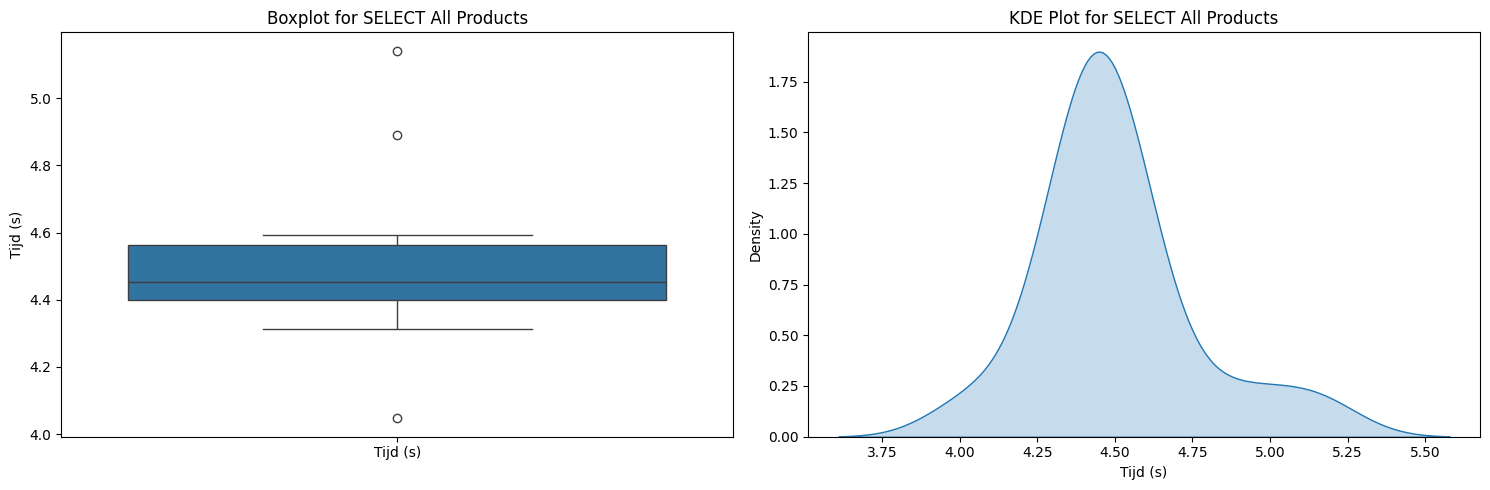
\includegraphics[width=\linewidth]{graphics/plots-slect-all-mariadb}
    \caption[Box- en KDE-plot select all MariaDB]{Box- en KDE-plot voor het ophalen van alle producten in MariaDB}
    \label{fig:plots-slect-all-mariadb}
\end{figure}

\begin{table}[htbp]
    \centering
    \caption{Gemiddelde tijden voor SELECT + JOIN + WHERE SQL-operaties}
    \begin{tabularx}{\textwidth}{*{8}{>{\centering\arraybackslash}X}c}
        \toprule
        \multicolumn{8}{c}{Tijd (s)} & Gemiddelde \\
        \midrule
        4,875 & 4,875 & 4,844 & 4,859 & 4,859 & 4,844 & 4,891 & 4,719 & 4,836 \\
        4,922 & 4,781 & 4,875 & 4,828 & 4,734 & 4,859 & 4,828 & & \\
        \bottomrule
    \end{tabularx}
\end{table}
\begin{figure}[H]
    \centering
    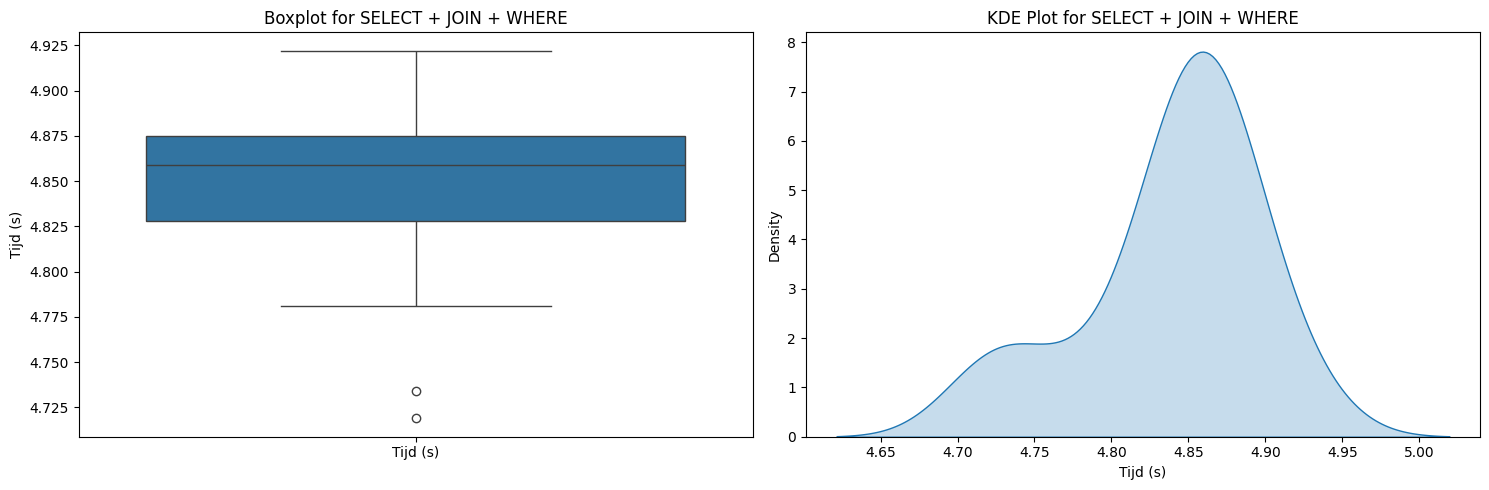
\includegraphics[width=\linewidth]{graphics/plots-slect-join-mariadb}
    \caption[Box- en KDE-plot select where MariaDB]{Box- en KDE-plot voor het selecteren van alle producten die vasthagen aan een bepaalde categorie in MariaDB}
    \label{fig:plots-slect-join-mariadb}
\end{figure}

\begin{table}[htbp]
    \centering
    \caption{Gemiddelde tijden voor BULK INSERT SQL-operaties}
    \begin{tabularx}{\textwidth}{*{8}{>{\centering\arraybackslash}X}c}
        \toprule
        \multicolumn{8}{c}{Tijd (s)} & Gemiddelde \\
        \midrule
        0,015 & 0,000 & 0,000 & 0,000 & 0,016 & 0,016 & 0,016 & 0,000 & 0,006 \\
        0,016 & 0,000 & 0,000 & 0,016 & 0,000 & 0,000 & 0,016 & & \\
        \bottomrule
    \end{tabularx}
\end{table}
\begin{figure}[H]
    \centering
    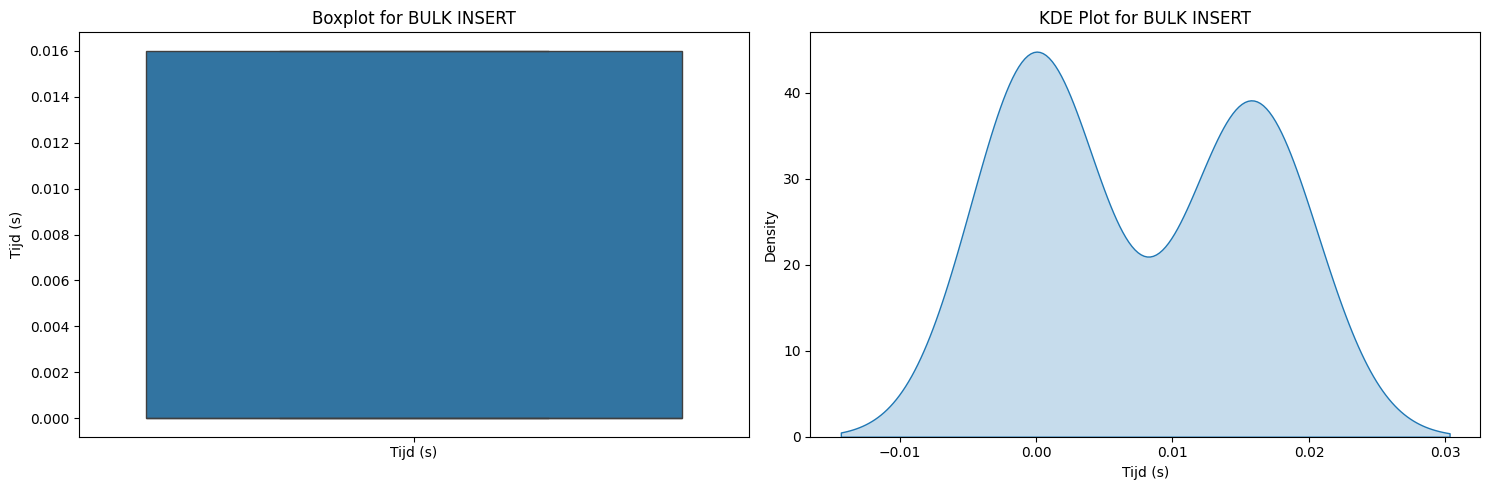
\includegraphics[width=\linewidth]{graphics/plots-insert-mariadb}
    \caption[Box- en KDE-plot insert MariaDB]{Box- en KDE-plot voor het toevoegen van een product in MariaDB}
    \label{fig:plots-insert-mariadb}
\end{figure}

\begin{table}[htbp]
    \centering
    \caption{Gemiddelde tijden voor UPDATE + WHERE SQL-operaties}
    \begin{tabularx}{\textwidth}{*{8}{>{\centering\arraybackslash}X}c}
        \toprule
        \multicolumn{8}{c}{Tijd (s)} & Gemiddelde \\
        \midrule
        11,562 & 11,625 & 12,281 & 12,109 & 12,375 & 12,109 & 12,359 & 11,406 & 11,865 \\
        12,141 & 11,250 & 11,765 & 11,875 & 12,141 & 11,734 & 11,473 & & \\
        \bottomrule
    \end{tabularx}
\end{table}
\begin{figure}[H]
    \centering
    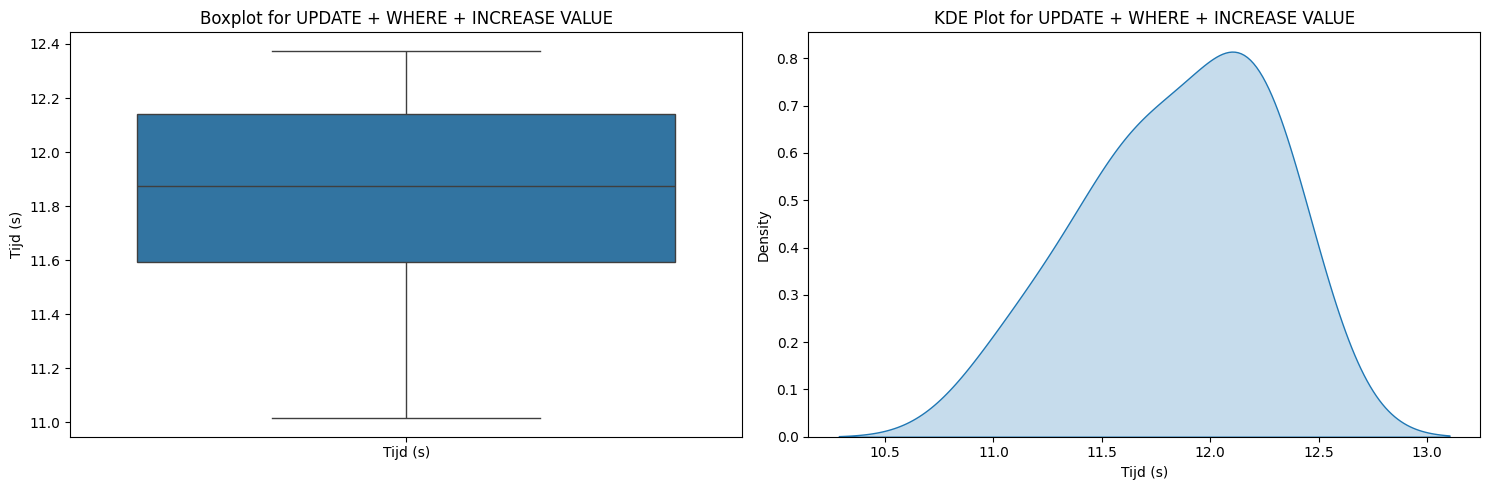
\includegraphics[width=\linewidth]{graphics/plots-update-mariadb}
    \caption[Box- en KDE-plot update where MariaDB]{Box- en KDE-plot voor het verhogen van een waarde van een product in MariaDB}
    \label{fig:plots-update-mariadb}
\end{figure}

\begin{table}[htbp]
    \centering
    \caption{Gemiddelde tijden voor DELETE SQL-operaties}
    \begin{tabularx}{\textwidth}{*{8}{>{\centering\arraybackslash}X}c}
        \toprule
        \multicolumn{8}{c}{Tijd (s)} & Gemiddelde \\
        \midrule
        0,015 & 0,000 & 0,000 & 0,000 & 0,000 & 0,000 & 0,000 & 0,015 & 0,004 \\
        0,000 & 0,000 & 0,000 & 0,000 & 0,015 & 0,015 & 0,000 & & \\
        \bottomrule
    \end{tabularx}
\end{table}

\begin{figure}[H]
    \centering
    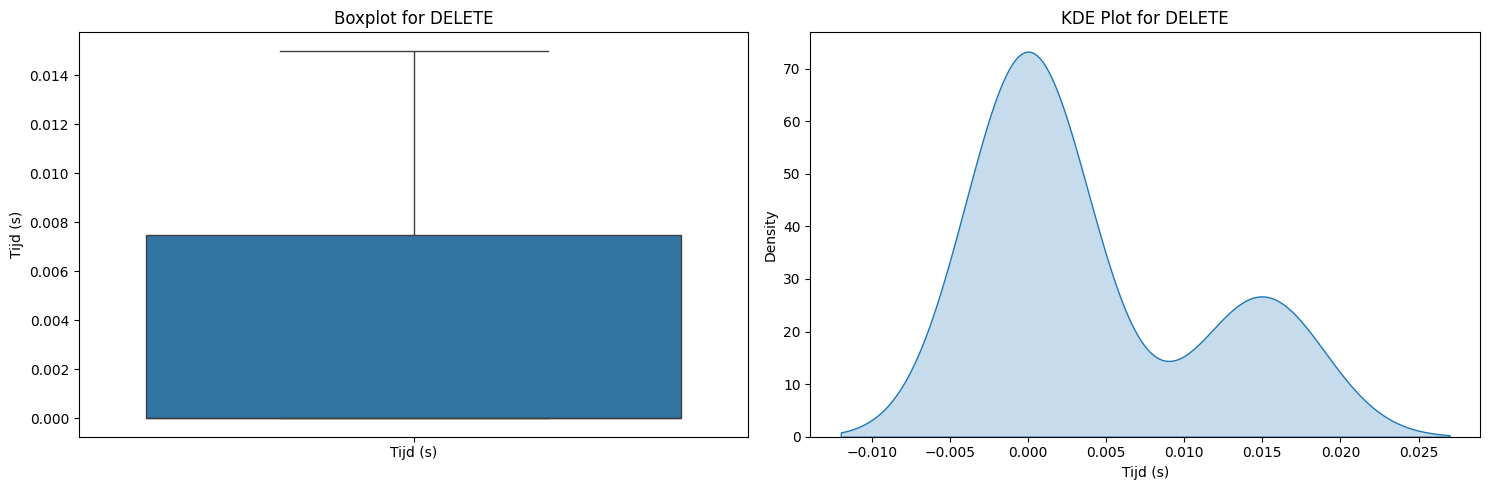
\includegraphics[width=\linewidth]{graphics/plots-delete-mariadb}
    \caption[Box- en KDE-plot delete MariaDB]{Box- en KDE-plot voor het verwijderen van een product in MariaDB}
    \label{fig:plots-delete-mariadb}
\end{figure}


\newpage




\section{\IfLanguageName{dutch}{MongoDB}{MongoDB}}%
\label{sec:test-mongodb}

\subsection{\IfLanguageName{dutch}{Opzetten database}{Creating database}}%
\label{subsec:creating-mongodb}

Voor het opzetten van de MongoDB-database is de bestaande data uit de MariaDB-database geëxporteerd naar een CSV-bestand. Enkel een deel van deze data kon geexporteerd worden alvorens een error optrad. ($\pm$ 1.9 miljoen rijen) Dit bestand is vervolgens geïmporteerd in het vooraf geïnstalleerde MongoDB Compass-programma. Vanwege de beperkte opslagcapaciteit van de gratis ter beschikking gestelde database kon slechts een deel van de gegevens worden geïmporteerd. ($\pm$ 1.5 miljoen rijen) Dit kan leiden tot afwijkingen in de gemeten data ten opzichte van onder andere de resultaten van MariaDB. Ondanks deze beperking kunnen de verkregen resultaten nog steeds nuttig zijn.

Figuur \ref{fig:mongodbsetup} toont de setup van de MongoDB-database, waarin de opslaggrootte van 52.6 MB, de logische gegevensgrootte, en het aantal documenten te zien zijn.

\begin{figure}[H]
    \centering
    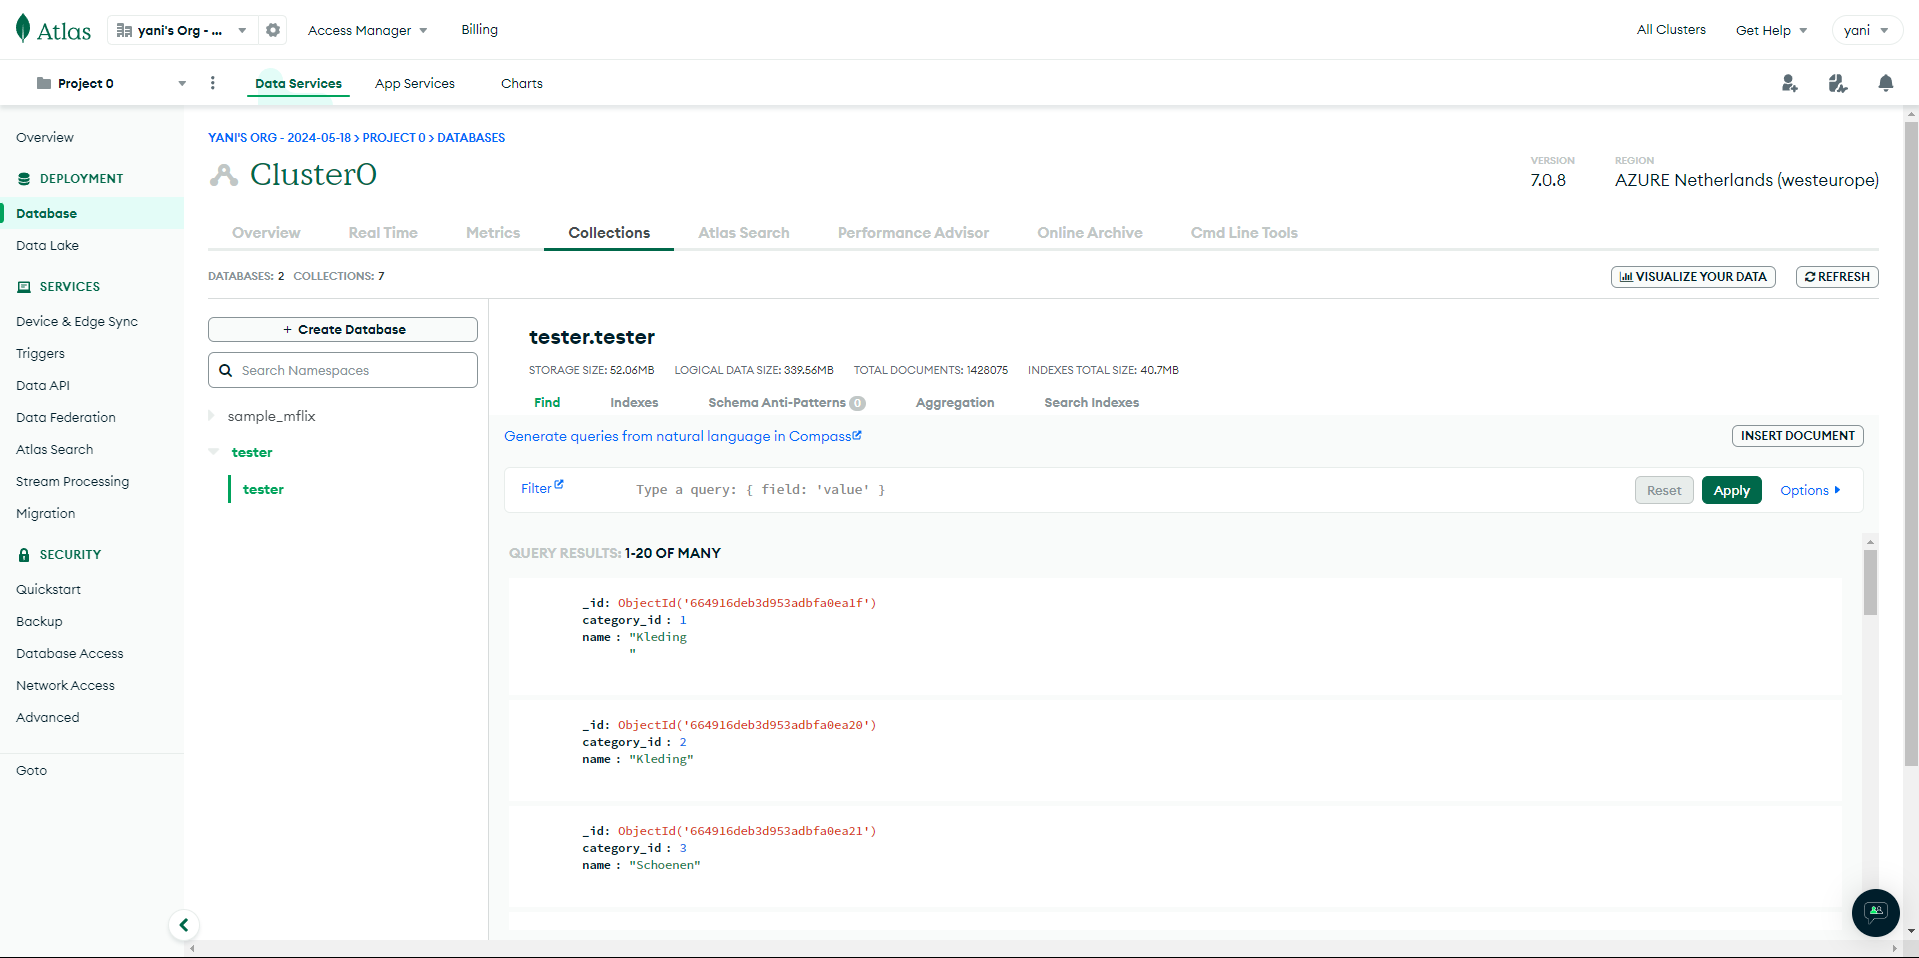
\includegraphics[width=\linewidth]{graphics/mongodbsetup}
    \caption[MongoDB setup]{MongoDB setup}
    \label{fig:mongodbsetup}
\end{figure}

\newpage

Voor het bekomen van de resultaten werden enkele queries opgesteld. Hieronder worden enkele voorbeelden weergegeven:
\begin{lstlisting}[language=NOSQL, caption={MongoDB-queries voor het beheren van producten in de database.}]
    -- Query 1: Ophalen van alle producten voor een bepaalde categorie.
    {'category_id': 3}
    
    -- Query 2: Update van een product
    db.products.updateOne(
    { product_id: 1 },
    {
        $set: {
            description: 'Nieuwe beschrijving',
            price: 49.99,
            stock: 100
        }
    }
    );
    
    -- Query 3: Toevoegen van een nieuw product
    db.products.insertOne({
        category_id: 1,
        SKU: 'SKU123',
        description: 'Nieuw product',
        price: 39.99,
        stock: 50,
        image: 'product_image.jpg',
        variations: {
            size: 'L',
            color: 'blue'
        }
    });
    
    -- Query 4: Verwijderen van een product
    db.products.deleteOne({ product_id: 2 });
\end{lstlisting}

\newpage

\subsection{\IfLanguageName{dutch}{Resultaten}{Results}}%
\label{subsec:results2}

Na het uitvoeren van de verschillende queries werden voor MongoDB volgende resultaten verkregen:

\begin{table}[htbp]
    \centering
    \caption{Gemiddelde tijden voor SELECT all - {}}
    \begin{tabularx}{\textwidth}{*{8}{>{\centering\arraybackslash}X}c}
        \toprule
        \multicolumn{8}{c}{Tijd (s)} & Gemiddelde \\
        \midrule
        0,977 & 0,945 & 0,929 & 0,921 & 0,997 & 0,940 & 0,926 & 1,050 & 0,964 \\
        0,950 & 0,910 & 0,835 & 0,864 & 1,036 & 0,825 & 0,865 & & \\
        \bottomrule
    \end{tabularx}
\end{table}

\begin{figure}[H]
    \centering
    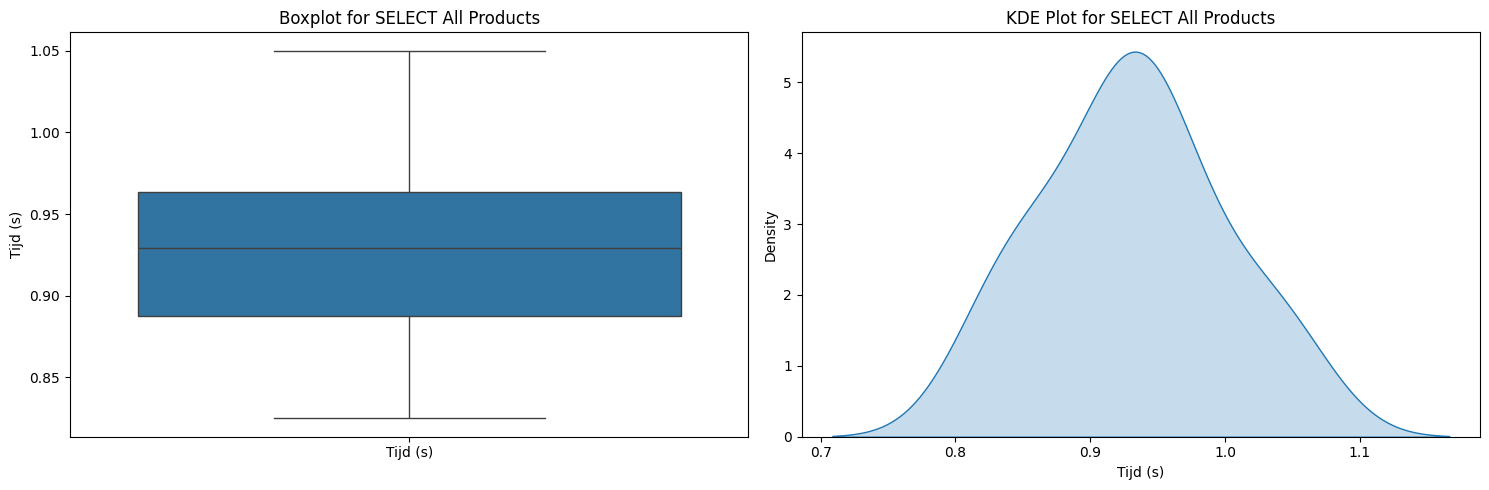
\includegraphics[width=\linewidth]{graphics/mongodb-select-all}
    \caption[Box- en KDE-plot select all MongoDB]{Box- en KDE-plot voor het selecteren van alle producten uit MongoDB.}
    \label{fig:mongodb-select-all}
\end{figure}


\begin{table}[htbp]
    \centering
    \caption{Gemiddelde tijden voor SELECT where - { "category_id": 3 }}
    \begin{tabularx}{\textwidth}{*{8}{>{\centering\arraybackslash}X}c}
        \toprule
        \multicolumn{8}{c}{Tijd (s)} & Gemiddelde \\
        \midrule
        1,399 & 1,509 & 1,385 & 1,288 & 1,289 & 1,386 & 1,291 & 1,270 & 1,353 \\
        1,272 & 1,265 & 1,362 & 1,454 & 1,271 & 1,284 & 1,253  & & \\
        \bottomrule
    \end{tabularx}
\end{table}

\begin{figure}[H]
    \centering
    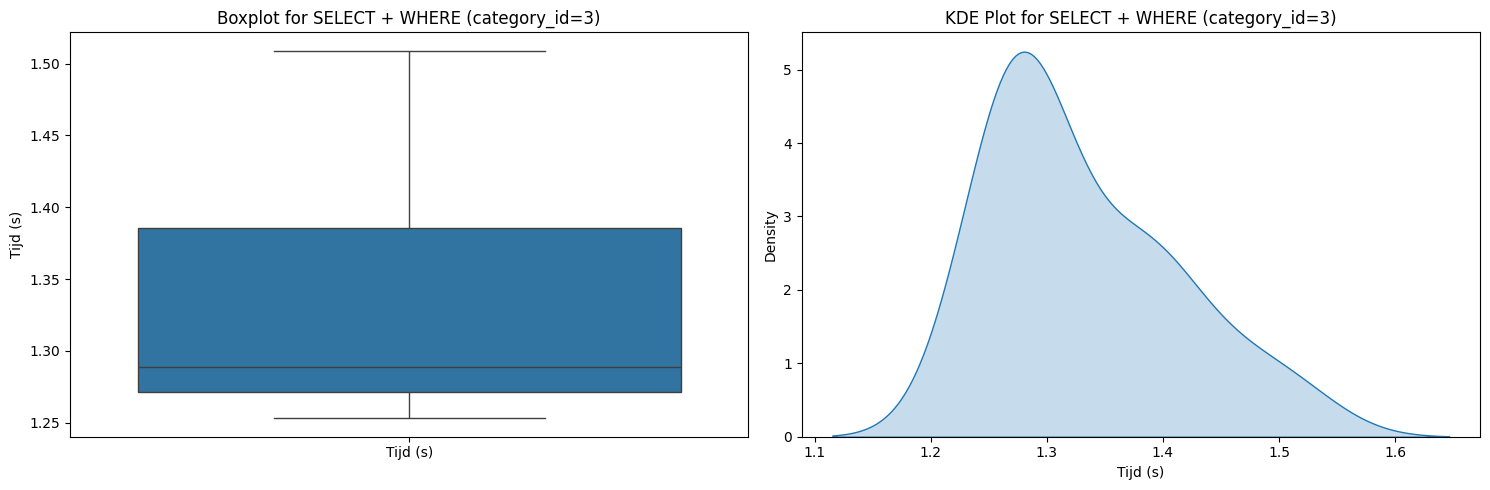
\includegraphics[width=\linewidth]{graphics/mongodb-select-category}
    \caption[Box- en KDE-plot select all where MongoDB]{Box- en KDE-plot voor het selecteren van alle producten waar de categorie id gelijk is aan 3 in MongoDB}
    \label{fig:mongodb-select-category}
\end{figure}

Voor MongoDB zijn er geen statistieken beschikbaar voor insert-, update- en delete-queries. Naast de maximale grootte van de database in de gratis versie, is er ook een beperking op het uitvoeren van bepaalde commando's. Een van deze commando's is het aanpassen van het profileringsniveau. Dit verhindert dat de uitvoeringssnelheid en andere statistieken van alle uitgevoerde queries beschikbaar worden gemaakt. Omdat gebruik werd gemaakt van de gratis versie, konden de querystatistieken alleen worden bekeken voor select-queries. In figuur \ref{fig:mongodberror} zijn het betreffende commando en de foutcode te vinden.

\begin{figure}[H]
    \centering
    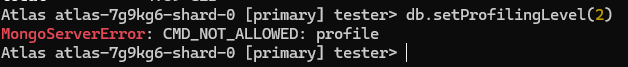
\includegraphics[width=\linewidth]{graphics/mongodberror}
    \caption[MongoDB foutcode]{MongoDB foutcode uitvoeren setProfilingLevel}
    \label{fig:mongodberror}
\end{figure}



\newpage



\section{\IfLanguageName{dutch}{Couchbase}{couchbase}}%
\label{sec:test-couchbase}

\subsection{\IfLanguageName{dutch}{Opzetten database}{Creating database}}%
\label{subsec:creating-couchbase}

Net zoals bij het opzetten van de MongoDB-database, werd voor het opzetten van de Couchbase-database een CSV-bestand gebruikt. Couchbase had echter een limiet op de grootte van deze bestanden, namelijk 40 MB. Dit betekende dat het slechts mogelijk was om maximaal 40 MB aan data te importeren.

\begin{figure}[H]
    \centering
    \includegraphics[width=\linewidth]{"graphics/Couchbase query"}
    \caption[Voorbeeld couchbase query]{Voorbeeld Couchbase query}
    \label{fig:couchbase-query}
\end{figure}

Figuur \ref{fig:couchbase-query} toont een screenshot van de Couchbase-datatools waarin de testen werden uitgevoerd. In de screenshot is ook een voorbeeld van een query te vinden, inclusief de uitvoeringstijd en hoe deze tijd wordt bepaald.

Hieronder volgen enkele gebruikte queries:

 \begin{lstlisting}[language=SQL, caption={Couchbase-queries voor het beheren van producten in de database.}]
     -- Query 1: Select all products
     SELECT * FROM fashion.`_default`.products;
     
     -- Query 2: Toevoegen van een product
     INSERT INTO `products` (KEY, VALUE)
     VALUES (UUID(), 
     {"c1": 2, "c2": "Home Appliances", "c3": "Refrigerators", 
         "c4": "Energy Efficient", "c5": 50,
          "c6": "Active", "c7": "2023-04-02", "c8": 300});
     
     -- Query 3: Updaten van een product
     UPDATE `products` SET c5 = c5 + 1 WHERE META().id = "3";
     
     -- Query 4: Verwijderen van een product
     DELETE FROM `products` WHERE META().id = "3";
 \end{lstlisting}


\subsection{\IfLanguageName{dutch}{Resultaten}{Results}}%
\label{subsec:results3}

Na het uitvoeren van de verschillende queries werden voor Couchbase volgende resultaten verkregen.

\begin{table}[htbp]
    \centering
    \caption{Gemiddelde tijden voor SELECT * FROM fashion.\_default.categories}
    \begin{tabularx}{\textwidth}{*{8}{>{\centering\arraybackslash}X}c}
        \toprule
        \multicolumn{8}{c}{Tijd (s)} & Gemiddelde \\
        \midrule
        7.9 & 12.8 & 18.9 & 9.4 & 9.8 & 10.7 & 15.4 & 8.7 & 11.8 \\
        13.5 & 8.4 & 10.1 & 14.7 & 23.1 & 8.9 & 10.2 & & \\
        \bottomrule
    \end{tabularx}
\end{table}

\begin{figure}[H]
    \centering
    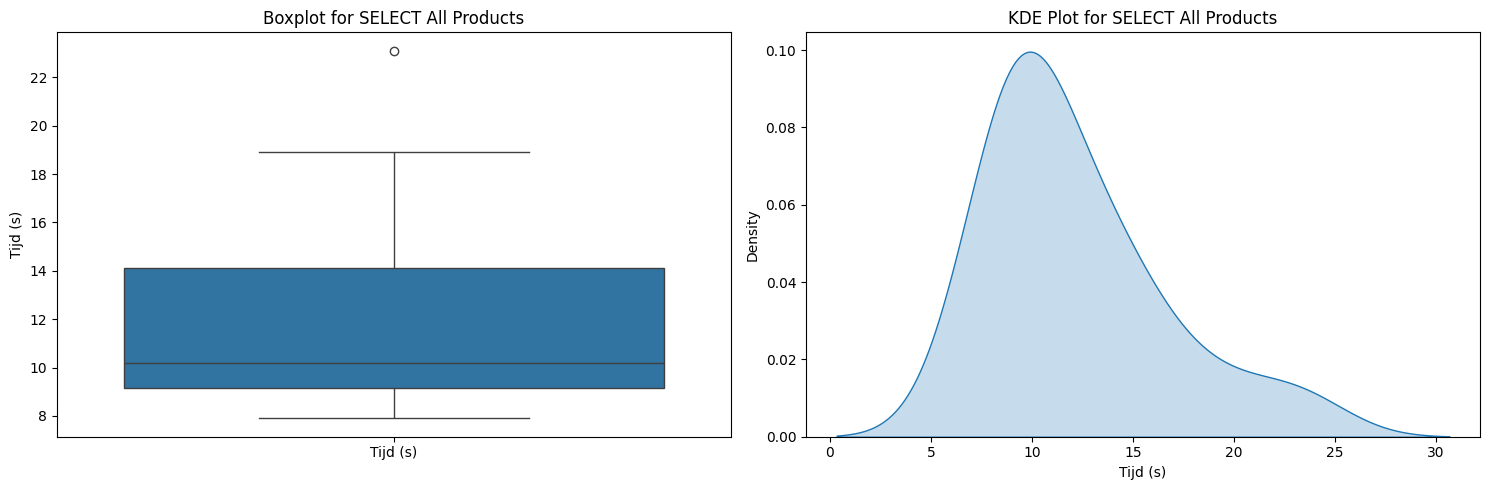
\includegraphics[width=\linewidth]{graphics/couchbase-select}
    \caption[Box- en KDE-plot select all Couchbase]{Box- en KDE-plot voor het selecteren van alle producten in Couchbase}
    \label{fig:couchbase-select}
\end{figure}


\begin{table}[htbp]
    \centering
    \caption{Gemiddelde tijden voor SELECT * FROM fashion.\_default.categories WHERE c8 = 3}
    \begin{tabularx}{\textwidth}{*{8}{>{\centering\arraybackslash}X}c}
        \toprule
        \multicolumn{8}{c}{Tijd (s)} & Gemiddelde \\
        \midrule
        7.0 & 7.8 & 9.7 & 7.7 & 8.6 & 13.0 & 10.8 & 8.3 & 8.8 \\
        7.9 & 7.9 & 8.5 & 9.9 & 9.7 & 11.2 & 6.5 & & \\
        \bottomrule
    \end{tabularx}
\end{table}

\begin{figure}[H]
    \centering
    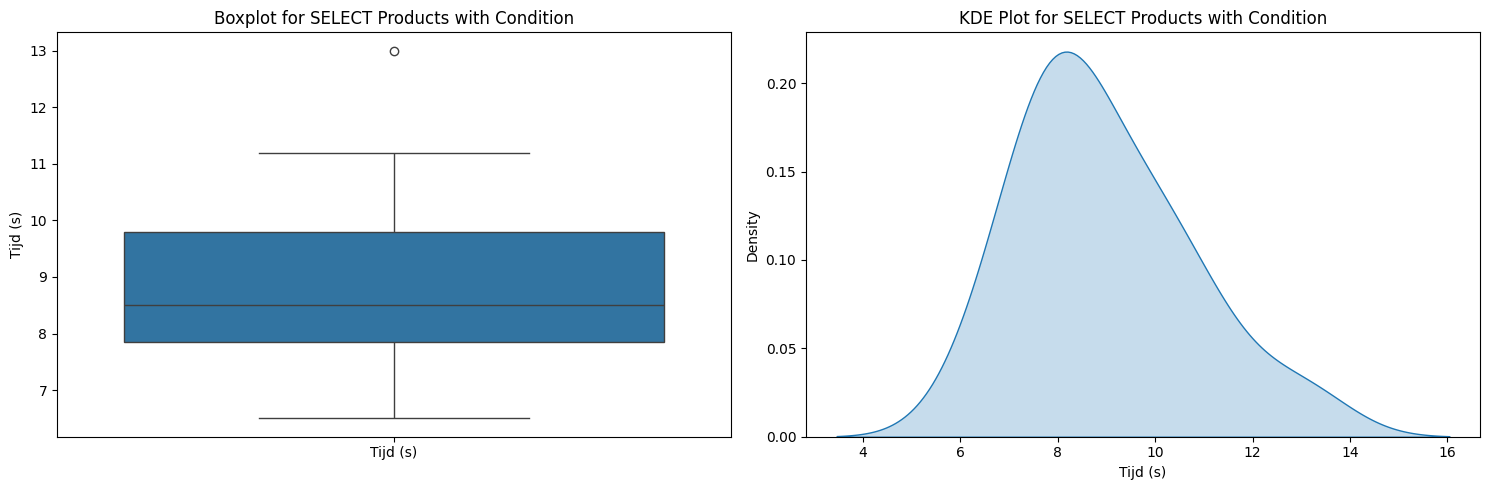
\includegraphics[width=\linewidth]{graphics/couchbase-select-where}
    \caption[Box- en KDE-plot select all where Couchbase]{Box- en KDE-plot voor het selecteren van alle producten die voldoen aan een bepaalde categorie id in Couchbase}
    \label{fig:couchbase-select-where}
\end{figure}


\begin{table}[htbp]
    \centering
    \caption{Gemiddelde tijden voor INSERT INTO categories}
    \begin{tabularx}{\textwidth}{*{8}{>{\centering\arraybackslash}X}c}
        \toprule
        \multicolumn{8}{c}{Tijd (s)} & Gemiddelde \\
        \midrule
        0.0017 & 0.0017 & 0.0014 & 0.0017 & 0.0016 & 0.0020 & 0.0020 & 0.0017 & 0.0017 \\
        0.0018 & 0.0017 & 0.0018 & 0.0018 & 0.0020 & 0.0016 & & \\
        \bottomrule
    \end{tabularx}
\end{table}

\begin{figure}[H]
    \centering
    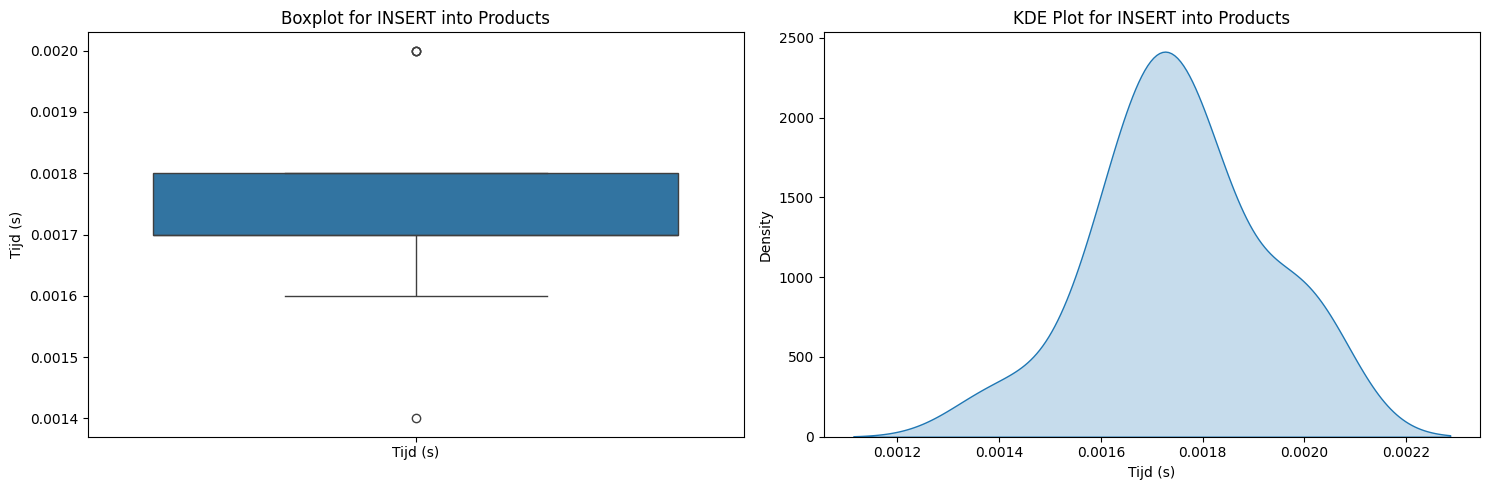
\includegraphics[width=\linewidth]{graphics/couchbase-insert}
    \caption[Box- en KDE-plot insert Couchbase]{Box- en KDE-plot voor het toevoegen van een product in Couchbase}
    \label{fig:couchbase-insert}
\end{figure}


\begin{table}[htbp]
    \centering
    \caption{Gemiddelde tijden voor UPDATE categories}
    \begin{tabularx}{\textwidth}{*{8}{>{\centering\arraybackslash}X}c}
        \toprule
        \multicolumn{8}{c}{Tijd (s)} & Gemiddelde \\
        \midrule
        0.0027 & 0.0024 & 0.0044 & 0.0030 & 0.0025 & 0.0022 & 0.0025 & 0.0026 & 0.0027 \\
        0.0021 & 0.0021 & 0.0026 & 0.0021 & 0.0023 & 0.0021 & & \\
        \bottomrule
    \end{tabularx}
\end{table}

\begin{figure}[H]
    \centering
    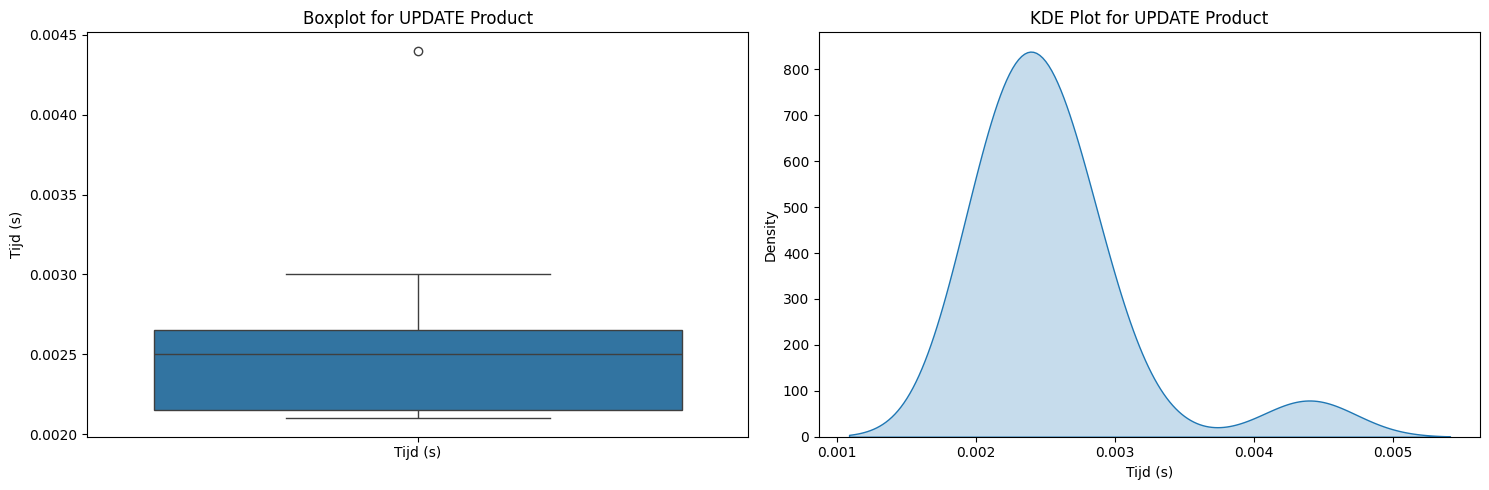
\includegraphics[width=\linewidth]{graphics/couchbase-update}
    \caption[Box- en KDE-plot update Couchbase]{Box- en KDE-plot voor het verhogen van een waarde van een product in Couchbase}
    \label{fig:couchbase-update}
\end{figure}

\begin{table}[htbp]
    \centering
    \caption{Gemiddelde tijden voor DELETE FROM categories}
    \begin{tabularx}{\textwidth}{*{8}{>{\centering\arraybackslash}X}c}
        \toprule
        \multicolumn{8}{c}{Tijd (s)} & Gemiddelde \\
        \midrule
        0.0044 & 0.0017 & 0.0017 & 0.0018 & 0.0018 & 0.0017 & 0.0018 & 0.0018 & 0.0021 \\
        0.0017 & 0.0018 & 0.0014 & 0.0022 & 0.0018 & 0.0017 & & \\
        \bottomrule
    \end{tabularx}
\end{table}

\begin{figure}[H]
    \centering
    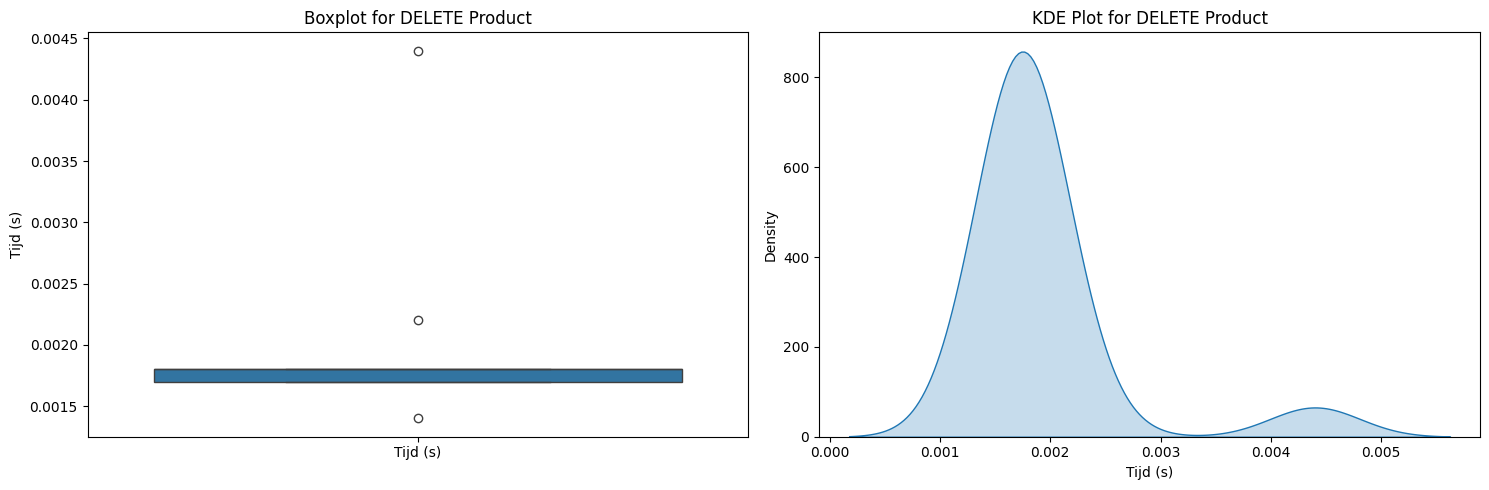
\includegraphics[width=\linewidth]{graphics/couchbase-delete}
    \caption[Box- en KDE-plot delete Couchbase]{Box- en KDE-plot voor het verwijderen van een product in Couchbase}
    \label{fig:couchbase-delete}
\end{figure}


\newpage

\section{\IfLanguageName{dutch}{Amazon Aurora}{Amazon Aurora}}%
\label{sec:test-amazonaurora}

Voor Amazon Aurora zijn er geen technische testen uitgevoerd aangezien voor het opzetten van een database op AWS een creditcard vereist was en deze niet beschikbaar kon gesteld worden. Hierdoor konden de gewenste performance testen en vergelijkingen met andere databases niet worden uitgevoerd.



\section{\IfLanguageName{dutch}{ClickHouse}{ClickHouse}}%
\label{sec:clickhouse}

\subsection{\IfLanguageName{dutch}{Opzetten database}{Creating database}}%
\label{subsec:creating-clickhouse}

Net zoals bij de andere databases, met uitzondering van MariaDB, werd voor het vullen van de ClickHouse-database een CSV-bestand gebruikt met eerder verzamelde data. ($\pm$ 1.9 miljoen rijen) Voor het uitvoeren van de queries is gebruik gemaakt van de Command Line Interface (CLI) die ClickHouse ter beschikking stelt. Dit zorgt ervoor dat nauwkeurige gegevens over de uitgevoerde queries makkelijk kunnen worden verzameld en geanalyseerd.

\begin{figure}[H]
    \centering
    \includegraphics[width=\linewidth]{"graphics/ClickHouse Query"}
    \caption[Voorbeeld query ClickHouse]{Voorbeeld query ClickHouse}
    \label{fig:clickhouse-query}
\end{figure}

Figuur \ref{fig:clickhouse-query} toont een screenshot van de ClickHouse CLI waarin een SELECT-query is uitgevoerd. Onder de gevonden resultaten kan meer informatie worden gevonden over de uitgevoerde query, zoals bijvoorbeeld de querysnelheid, het aantal gevonden rijen, en andere relevante details.


\newpage
Hieronder volgen enkele gebruikte queries:

\begin{lstlisting}[language=SQL, caption={Couchbase-queries voor het beheren van producten in de database.}]
    -- Query 1: Select all products
    SELECT * FROM producten;
    
    -- Query 2: Toevoegen van een categorie
    INSERT INTO categories (c1, c2) 
    VALUES ('new_category', 'new_description');
    
    -- Query 3: Updaten van een product
    ALTER TABLE producten 
    UPDATE c5 = toString(toUInt32(c5) + 1) WHERE c1 = '1'
    
    -- Query 4: Verwijderen van een categorie
    DELETE FROM categories 
    WHERE c1 = 'new_category' AND c2 = 'new_description';
\end{lstlisting}


\subsection{\IfLanguageName{dutch}{Resultaten}{Results}}%
\label{subsec:results5}

Na het uitvoeren van de verschillende queries werden voor ClickHouse volgende resultaten verkregen:

% Table for SELECT * FROM producten
\begin{table}[htbp]
    \centering
    \caption{Gemiddelde tijden voor SELECT * FROM producten}
    \begin{tabularx}{\textwidth}{*{8}{>{\centering\arraybackslash}X}c}
        \toprule
        \multicolumn{8}{c}{Tijd (s)} & Gemiddelde \\
        \midrule
        0.307 & 0.243 & 0.243 & 0.240 & 0.277 & 0.250 & 0.255 & 0.236 & 0.261 \\
        0.243 & 0.264 & 0.263 & 0.235 & 0.282 & 0.253 & 0.293 & & \\
        \bottomrule
    \end{tabularx}
\end{table}

\begin{figure}[H]
    \centering
    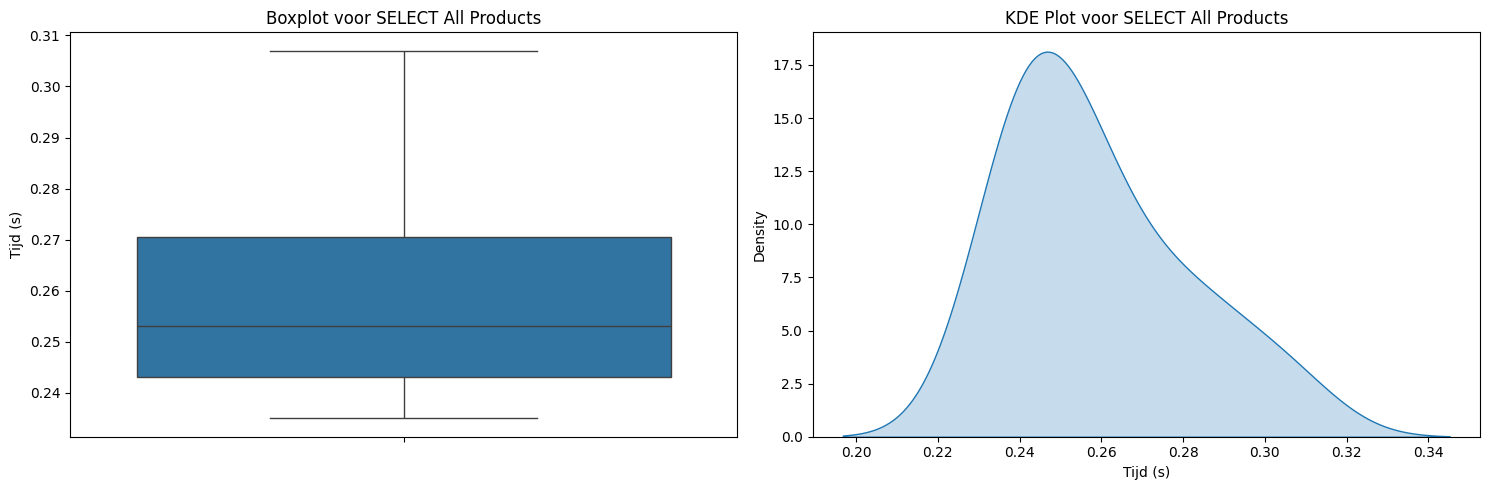
\includegraphics[width=\linewidth]{graphics/clickhouse-all}
    \caption[Box- en KDE-plot select all ClickHouse]{Box- en KDE-plot voor het selecteren van alle producten in ClickHouse}
    \label{fig:clickhouse-all}
\end{figure}


% Table for SELECT * FROM producten INNER JOIN categories
\begin{table}[htbp]
    \centering
    \caption{Gemiddelde tijden voor SELECT * FROM producten INNER JOIN categories}
    \begin{tabularx}{\textwidth}{*{8}{>{\centering\arraybackslash}X}c}
        \toprule
        \multicolumn{8}{c}{Tijd (s)} & Gemiddelde \\
        \midrule
        0.383 & 0.365 & 0.391 & 0.466 & 0.411 & 0.432 & 0.389 & 0.379 & 0.397 \\
        0.367 & 0.434 & 0.423 & 0.382 & 0.424 & 0.340 & 0.362 & & \\
        \bottomrule
    \end{tabularx}
\end{table}
\begin{figure}[H]
    \centering
    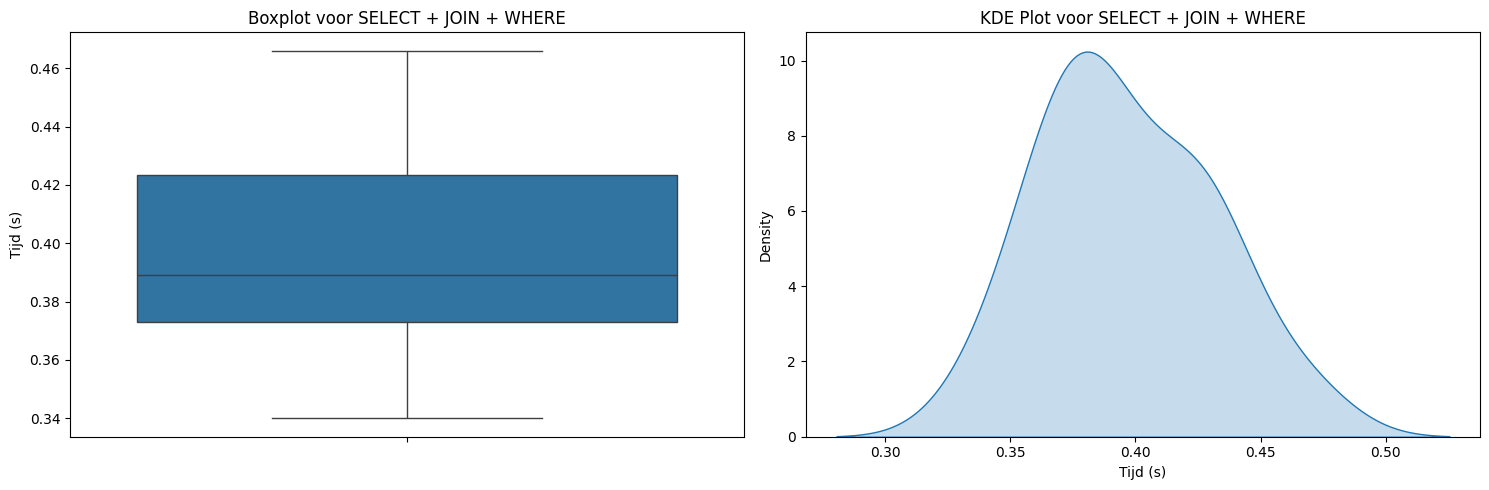
\includegraphics[width=\linewidth]{graphics/clickhouse-all-where}
    \caption[Box- en KDE-plot select all where ClickHouse]{Box- en KDE-plot voor het selecteren van alle producten die voldoen aan een bepaalde categorie id in ClickHouse}
    \label{fig:clickhouse-all-where}
\end{figure}

% Table for INSERT INTO producten
\begin{table}[htbp]
    \centering
    \caption{Gemiddelde tijden voor INSERT INTO producten}
    \begin{tabularx}{\textwidth}{*{8}{>{\centering\arraybackslash}X}c}
        \toprule
        \multicolumn{8}{c}{Tijd (s)} & Gemiddelde \\
        \midrule
        0.065 & 0.072 & 0.060 & 0.081 & 0.095 & 0.071 & 0.098 & 0.078 & 0.078 \\
        0.074 & 0.072 & 0.086 & 0.082 & 0.096 & 0.101 & 0.065 & & \\
        \bottomrule
    \end{tabularx}
\end{table}

\begin{figure}[H]
    \centering
    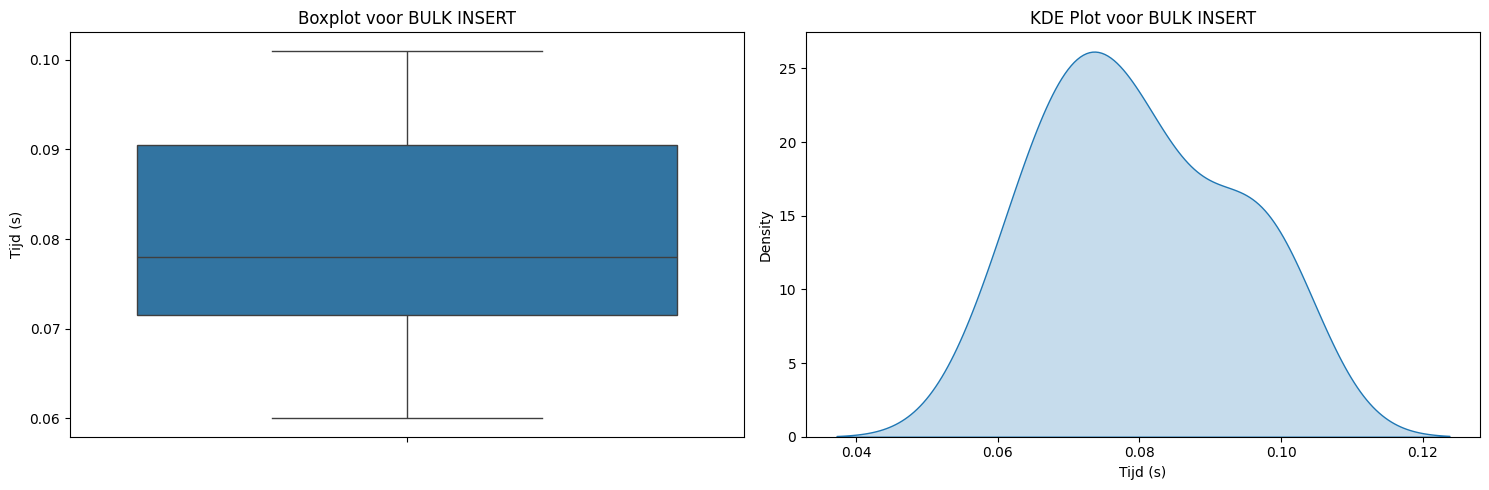
\includegraphics[width=\linewidth]{graphics/clickhouse-bulk-insert}
    \caption[Box- en KDE-plot insert ClickHouse]{Box- en KDE-plot voor het toevoegen van een product in ClickHouse}
    \label{fig:clickhouse-bulk-insert}
\end{figure}


% Table for UPDATE producten SET c5
\begin{table}[htbp]
    \centering
    \caption{Gemiddelde tijden voor UPDATE producten SET c5}
    \begin{tabularx}{\textwidth}{*{8}{>{\centering\arraybackslash}X}c}
        \toprule
        \multicolumn{8}{c}{Tijd (s)} & Gemiddelde \\
        \midrule
        0.056 & 0.059 & 0.058 & 0.057 & 0.054 & 0.054 & 0.055 & 0.058 & 0.055 \\
        0.057 & 0.054 & 0.055 & 0.055 & 0.054 & 0.053 & 0.053 & & \\
        \bottomrule
    \end{tabularx}
\end{table}

\begin{figure}[H]
    \centering
    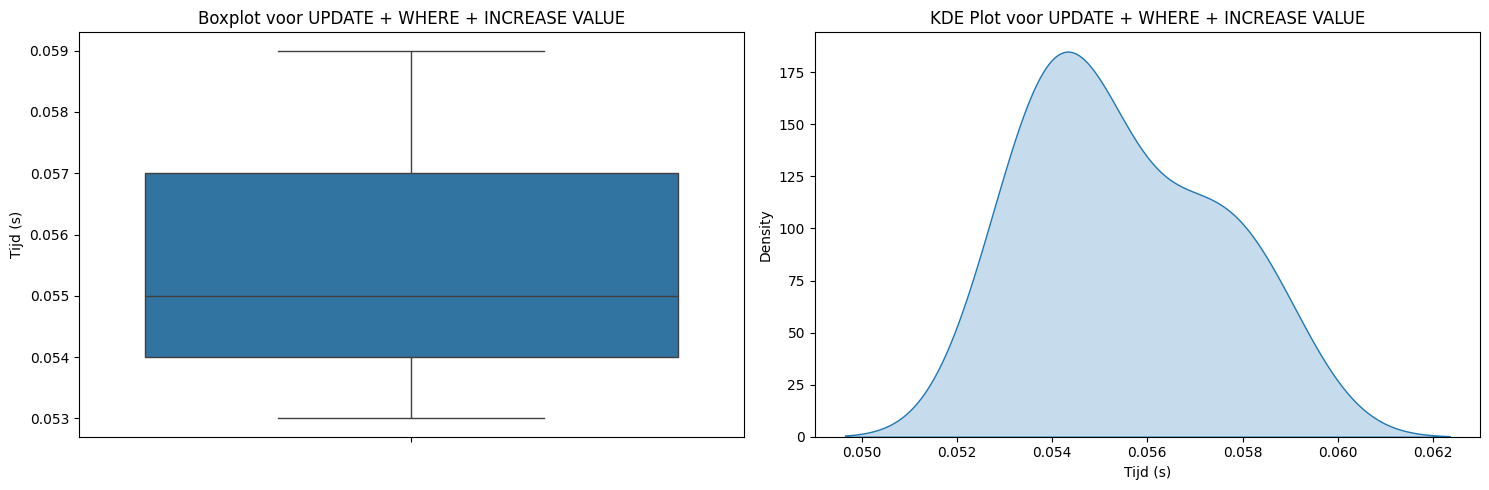
\includegraphics[width=\linewidth]{graphics/clickhouse-update}
    \caption[Box- en KDE-plot update ClickHouse]{Box- en KDE-plot voor het verhogen van een waarde van een product in ClickHouse}
    \label{fig:clickhouse-update}
\end{figure}


% Table for DELETE FROM categories
\begin{table}[htbp]
    \centering
    \caption{Gemiddelde tijden voor DELETE FROM categories}
    \begin{tabularx}{\textwidth}{*{8}{>{\centering\arraybackslash}X}c}
        \toprule
        \multicolumn{8}{c}{Tijd (s)} & Gemiddelde \\
        \midrule
        0.126 & 0.125 & 0.128 & 0.151 & 0.130 & 0.131 & 0.117 & 0.128 & 0.129 \\
        0.130 & 0.132 & 0.129 & 0.135 & 0.120 & 0.143 & 0.130 & & \\
        \bottomrule
    \end{tabularx}
\end{table}

\begin{figure}[H]
    \centering
    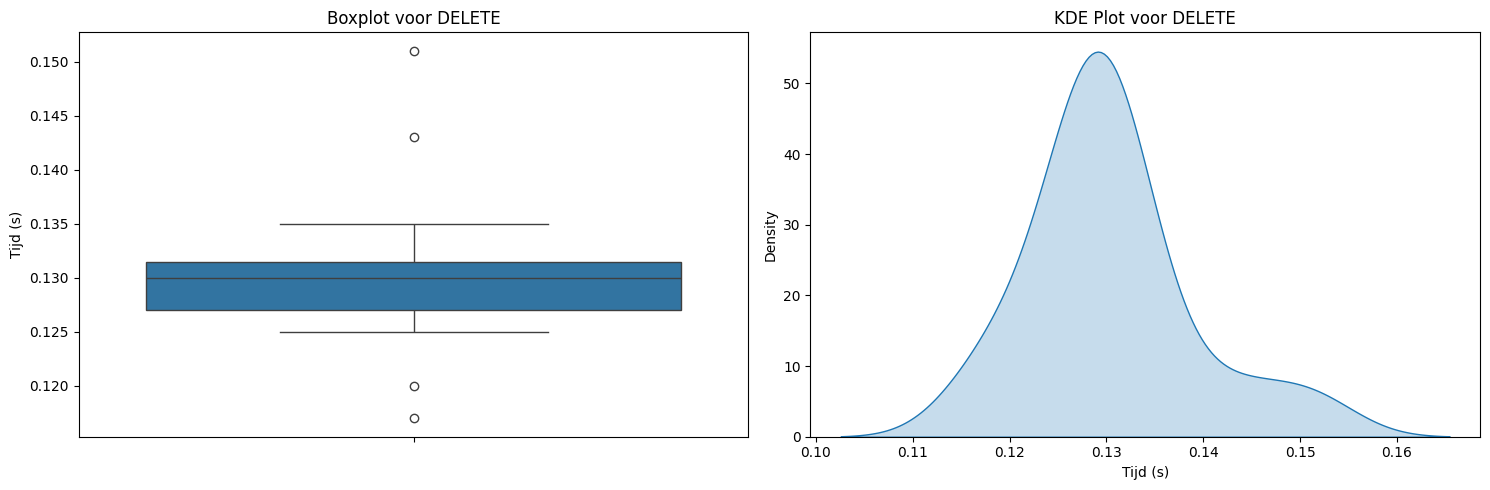
\includegraphics[width=\linewidth]{graphics/clickhouse-delete}
    \caption[Box- en KDE-plot delete ClickHouse]{Box- en KDE-plot voor het verwijderen van een product in ClickHouse}
    \label{fig:clickhouse-delete}
\end{figure}



\newpage


\section{\IfLanguageName{dutch}{Conclusie}{Conclusie}}%
\label{sec:test-conclusie}

Aan de hand van de verzamelde resultaten van MariaDB, MongoDB, Couchbase en Clickhouse kunnen de prestaties met elkaar vergeleken worden. De gemiddelde tijden voor elke uitgevoerde operatie geven een beter inzicht in de efficiëntie en snelheid van elk van deze databases. Het is echter belangrijk om te vermelden dat niet alle resultaten 100\% betrouwbaar zijn. Veel van de uitgevoerde queries werden uitgevoerd in de cloud. Dit zorgt ervoor dat verschillende factoren zoals bijvoorbeeld netwerkvertragingen en serverbelasting de resultaten kunnen beïnvloeden. Daarnaast werd ook niet evenveel data gebruikt voor elk van deze databases vanwege de beperkingen die werden opgelegd door de free trials. Bovendien kon de Amazon Aurora database niet getest worden wegens het ontbreken van een creditcard voor het opzetten van deze database. Ondanks de hierboven beschreven beperkingen worden hieronder de belangrijkste conclusies uit de resultaten weergegeven.

\vspace{5mm}

Wat betreft het ophalen van gegevens blijkt uit de resultaten dat ClickHouse de beste prestaties biedt met een respectief gemiddelde van 0.261 en 0.397 seconden. Daarna komen MongoDB met 0.964 en 1.353 seconden en MariaDB met 4.479 en 4.836 seconden. Couchbase scoorde het slechtst met een gemiddelde van maar liefst 11.8 en 8.8 seconden. Het is nogmaals belangrijk om te melden dat MariaDB de meeste data gebruikt heeft voor deze metingen. Uit deze gemiddelde berekeningen kan besloten worden dat hoewel meer data gebruikt was voor de MariaDB database, ClickHouse mogelijks de betere database is voor het ophalen van grote hoeveelheden aan gegevens. 

\vspace{5mm}

Een database moet echter meer doen dan enkel gegevens ophalen. Ze moeten ook in staat zijn om snel gegevens op te slaan, te verwijderen en bij te werken. Voor het toevoegen van gegevens scoort Couchbase het best.

Ook voor het verwijderen van gegevens heeft Couchbase de beste resultaten. Na Couchbase volgen MariaDB, MongoDB en ClickHouse in hun respectievelijke volgorde.

Voor het updaten van de gegevens scoort MariaDB het slechts met een gemiddelde tijd van 11.865 seconden. Dit is aanzienlijk meer dan de gemiddelde tijden van zowel Couchbase, ClickHouse en MongoDB. OOk hier scoort Couchbase het best. 

\vspace{5mm}

Het is echter belangrijk om te benadrukken dat de betrouwbaarheid van deze resultaten beïnvloed kan zijn door verschillende factoren in de cloudomgeving, zoals:
\begin{itemize}
    \item \textbf{Netwerkvertragingen}: Variaties in de netwerk latency kunnen de responstijden beïnvloeden.
    \item \textbf{Serverbelasting}: De belasting op de servers tijdens het uitvoeren van de queries kan de prestaties beïnvloeden.
    \item \textbf{Resourcebeschikbaarheid}: Fluctuaties in de beschikbaarheid van CPU, geheugen en opslag kunnen de prestaties variëren.
    \item \textbf{Geografische locatie van de servers}: Afstanden tussen de servers en de clients kunnen de netwerkvertragingen verhogen.
\end{itemize}

\vspace{5mm}

Op basis van de gevonden resultaten en rekening houdende met de verschillende factoren kan besloten worden dat voor het uitvoeren van lees-intensieve operaties (SELECT) Clickhouse de beste prestaties biedt. Voor schrijf-intensieve operaties (INSERT en UPDATE) presteert Couchbase zeer goed, hoewel MariaDB en Clickhouse ook competitief zijn. MariaDB blinkt uit bij BULK INSERT operaties. Over het algemeen lijkt Clickhouse de beste oplossing voor een e-commerce webshop in de mode-industrie. Het is belangrijk om de genoemde factoren in de cloudomgeving mee in overweging te nemen bij het interpreteren van deze resultaten.